%==============================================================================
% EULER'S MATHEMATICS: A Comprehensive Reference
%==============================================================================
\documentclass[11pt,a4paper,twoside]{book}

\usepackage[utf8]{inputenc}
\usepackage[T1]{fontenc}
\usepackage{lmodern}
\usepackage{microtype}
\usepackage{amsmath,amsthm,amssymb}
\usepackage{mathtools}
\usepackage{graphicx}
\usepackage{xcolor}
\usepackage{hyperref}
\usepackage{booktabs}
\usepackage{array}
\usepackage{geometry}
\usepackage{fancyhdr}
\usepackage{titlesec}
\usepackage{epigraph}
\usepackage{float}
\usepackage{caption}
\usepackage{subcaption}
\usepackage{makeidx}
\usepackage{doi}
\usepackage{bookmark}

\geometry{
    paper=a4paper,
    inner=30mm,
    outer=25mm,
    top=30mm,
    bottom=30mm,
    headheight=48pt,
    headsep=10mm,
    footskip=12mm,
    marginparwidth=20mm,
}

\definecolor{eulerblue}{RGB}{0, 51, 102}
\definecolor{eulerdark}{RGB}{0, 30, 60}

\hypersetup{
    colorlinks=true,
    linkcolor=eulerblue,
    citecolor=eulerblue,
    urlcolor=eulerblue,
    pdfauthor={Euler Mathematics Project},
    pdftitle={Euler's Mathematics: A Comprehensive Reference},
    pdfsubject={Mathematics / History of Mathematics},
    pdfkeywords={Euler, number theory, analysis, graph theory, complex analysis, special functions},
}

\newtheoremstyle{eulerstyle}
    {1em}{1em}{\itshape}{}{\bfseries}{.}{0.5em}{}
\theoremstyle{eulerstyle}
\newtheorem{theorem}{Theorem}[chapter]
\newtheorem{lemma}[theorem]{Lemma}
\newtheorem{corollary}[theorem]{Corollary}
\newtheorem{proposition}[theorem]{Proposition}
\newtheorem{conjecture}[theorem]{Conjecture}

\theoremstyle{definition}
\newtheorem{definition}[theorem]{Definition}
\newtheorem{example}[theorem]{Example}
\newtheorem{historical}[theorem]{Historical Note}
\newtheorem{application}[theorem]{Application}
\newtheorem{remark}[theorem]{Remark}

\titleformat{\chapter}[display]
    {\normalfont\huge\bfseries\color{eulerblue}}
    {\chaptername\ \thechapter}
    {20pt}
    {\Huge}
    [{\color{eulerblue}\titlerule[2pt]}]

\titleformat{\section}
    {\normalfont\Large\bfseries\color{eulerblue}}
    {\thesection}{1em}{}
    
\titleformat{\subsection}
    {\normalfont\large\bfseries\color{eulerdark}}
    {\thesubsection}{1em}{}

\pagestyle{fancy}
\fancyhf{}
\fancyhead[LE]{\thepage\quad\leftmark}
\fancyhead[RO]{\rightmark\quad\thepage}
\fancyfoot[C]{}
\renewcommand{\headrulewidth}{0.5pt}
\renewcommand{\footrulewidth}{0pt}

\newcommand{\Z}{\mathbb{Z}}
\newcommand{\N}{\mathbb{N}}
\newcommand{\R}{\mathbb{R}}
\newcommand{\C}{\mathbb{C}}
\newcommand{\Q}{\mathbb{Q}}
\newcommand{\p}{\mathbb{P}}
\DeclareMathOperator{\lcm}{lcm}
\DeclareMathOperator{\ord}{ord}
\DeclareMathOperator{\Li}{Li}
\DeclareMathOperator{\id}{id}
\newcommand{\ph}{\varphi}

\makeindex

\begin{document}

\frontmatter

\begin{titlepage}
    \centering
    \vspace*{2cm}
    
    {\Huge \color{eulerblue} Euler's Mathematics}\\[0.5cm]
    {\Large \color{eulerdark} A Comprehensive Reference}\\[1.5cm]
    
    \vspace{1cm}
    
    {\large Theory, History, Applications, and Theorems}\\[2cm]
    
    \vfill
    
    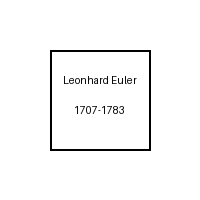
\includegraphics[width=0.4\textwidth]{figures/euler_portrait.png}\\[2cm]
    
    {\large \color{eulerblue} Leonhard Euler (1707--1783)}\\[1cm]
    
    \vfill
    
    {\large Euler Mathematics Project}\\[0.5cm]
    {\today}
    
    \vspace{1cm}
    
    {\small \textit{``Read Euler, read Euler, he is the master of us all.''}\\[0.2cm]
    --- Pierre-Simon Laplace}
\end{titlepage}

\cleardoublepage

\thispagestyle{empty}
\vspace*{\fill}
\noindent\textcopyright\ 2025 Euler Mathematics Project.\\[0.5cm]
This work is licensed under a Creative Commons Attribution-NonCommercial-ShareAlike 4.0 International License.\\[1cm]
\textbf{ISBN:} --- (to be assigned)\\[0.5cm]
Typeset with \LaTeX\ using the \texttt{book} class.

\cleardoublepage

\chapter*{Preface}
\addcontentsline{toc}{chapter}{Preface}

\epigraph{``Read Euler, read Euler, he is the master of us all.''}{--- Pierre-Simon Laplace}
\epigraph{``Euler calculated without apparent effort, as men breathe, or as eagles sustain themselves in the wind.''}{--- François Arago}

Leonhard Euler (1707--1783) is the most prolific mathematician in history. His collected works, the \emph{Opera Omnia}, span over 80 volumes. He introduced much of modern mathematical notation: $e$, $i$, $\pi$, $\sum$, $\prod$, $f(x)$, $\sin$, $\cos$, $\Gamma$, $\zeta$, $\Delta$, $\nabla$, and many more. His discoveries span number theory, analysis, graph theory, mechanics, astronomy, optics, and fluid dynamics.

This book is a comprehensive mathematical reference to Euler's work. It presents:
\begin{itemize}
    \item Complete statements of Euler's theorems with historical context
    \item Proofs and derivations where accessible
    \item Applications in modern mathematics and science
    \item Connections between different areas of Euler's work
    \item References to Euler's original papers (with Opera Omnia volume/page)
\end{itemize}

This is \textbf{not} a computational guide. For Python implementations, exercises, and computational experiments, see the companion volume \emph{Euler's Mathematics: A Computational Student Guide}.

\vspace{1cm}
\begin{flushright}
\textit{The Euler Mathematics Project}
\end{flushright}

\cleardoublepage

\tableofcontents

\cleardoublepage

\mainmatter

%==============================================================================
% PART I: NUMBER THEORY
%==============================================================================
\part{Number Theory and Arithmetic}
\label{part:number_theory}

%----------------------------------------------------------
% Chapter 1: Totient Function and Modular Arithmetic
%----------------------------------------------------------
\chapter{Euler's Totient Function and Modular Arithmetic}
\label{ch:totient}

\begin{historical}
Euler introduced the totient function $\varphi(n)$ in his 1763 paper \emph{Theoremata arithmetica nova methodo demonstrata} (Opera Omnia, Series I, Vol. 4, pp. 74--104). He proved the product formula and the theorem generalizing Fermat's little theorem. The notation $\varphi(n)$ was introduced by Gauss in 1801; Euler used $\pi n$ or simply $n$. \cite{euler1763}\end{historical}

\section{Definition and Basic Properties}

\begin{definition}[Euler's Totient Function]
For $n \in \N$, the \emph{totient function} $\varphi(n)$ counts the integers $1 \le k \le n$ with $\gcd(k,n)=1$:
\[
\varphi(n) = |\{k \in \Z : 1 \le k \le n,\ \gcd(k,n) = 1\}|.
\]
\end{definition}

\begin{theorem}[Product Formula for $\varphi(n)$]
If $n = p_1^{e_1} p_2^{e_2} \cdots p_r^{e_r}$ is the prime factorization, then
\[
\varphi(n) = n \prod_{i=1}^r \left(1 - \frac{1}{p_i}\right)
= \prod_{i=1}^r p_i^{e_i-1}(p_i - 1).
\]
\end{theorem}

\begin{theorem}[Multiplicativity]
If $\gcd(m,n)=1$, then $\varphi(mn) = \varphi(m)\varphi(n)$.
\end{theorem}

\begin{theorem}[Sum of Totients]
\[
\sum_{d|n} \varphi(d) = n.
\]
\end{theorem}

\section{Euler's Theorem and Applications}

\begin{theorem}[Euler's Theorem (1763)]
If $\gcd(a,n)=1$, then
\[
a^{\varphi(n)} \equiv 1 \pmod{n}.
\]
\end{theorem}

\begin{corollary}[Fermat's Little Theorem]
If $p$ is prime and $p \nmid a$, then $a^{p-1} \equiv 1 \pmod{p}$.
\end{corollary}

\begin{application}[RSA Cryptography]
The RSA cryptosystem uses $\varphi(n) = (p-1)(q-1)$ for $n=pq$ with $p,q$ prime. 
Encryption: $c \equiv m^e \pmod{n}$; Decryption: $m \equiv c^d \pmod{n}$ where $ed \equiv 1 \pmod{\varphi(n)}$.
\end{application}

\begin{application}[Primitive Roots]
A primitive root modulo prime $p$ is a generator of $(\Z/p\Z)^\times$. There are $\varphi(p-1)$ primitive roots modulo $p$.
\end{application}

\begin{application}[Cyclotomic Polynomials]
The $n$-th cyclotomic polynomial $\Phi_n(x)$ has degree $\varphi(n)$ and satisfies
\[
x^n - 1 = \prod_{d|n} \Phi_d(x).
\]
\end{application}

\section{Asymptotic Behavior}

\begin{theorem}[Euler's Result on Totient Sums]
\[
\sum_{k=1}^n \varphi(k) = \frac{3}{\pi^2} n^2 + O(n \log n).
\]
\end{theorem}

This implies the probability that two random integers are coprime is
\[
\lim_{n \to \infty} \frac{1}{n^2} \sum_{k=1}^n \varphi(k) = \frac{6}{\pi^2} = \frac{1}{\zeta(2)}.
\]

\cleardoublepage

%----------------------------------------------------------
% Chapter 2: Prime Numbers and the Euler Product
%----------------------------------------------------------
\chapter{Prime Numbers and the Euler Product}
\label{ch:primes}

\begin{historical}
Euler's 1737 paper \emph{Variae observationes circa series infinitas} (Opera Omnia, Series I, Vol. 14, pp. 160--188) introduced the Euler product formula and proved the divergence of the sum of reciprocal primes, giving a new proof of the infinitude of primes. \cite{euler1737}\end{historical}

\section{Euler's Proof of Infinitely Many Primes}

\begin{theorem}[Euler, 1737]
The sum of reciprocals of primes diverges:
\[
\sum_{p \text{ prime}} \frac{1}{p} = \infty.
\]
\end{theorem}

\begin{proof}
Euler used the product formula for $\zeta(s)$:
\[
\zeta(s) = \prod_{p} \frac{1}{1 - p^{-s}} \qquad (s > 1).
\]
Taking logarithms and using $\log(1-x) \approx -x$ for small $x$:
\[
\log \zeta(s) = \sum_p \log \frac{1}{1-p^{-s}} = \sum_p \left( \frac{1}{p^s} + O\left(\frac{1}{p^{2s}}\right) \right).
\]
As $s \to 1^+$, $\zeta(s) \sim \frac{1}{s-1} \to \infty$, so $\sum_p 1/p^s \to \infty$. Hence $\sum_p 1/p$ diverges.
\end{proof}

\section{The Euler Product Formula}

\begin{theorem}[Euler Product for the Zeta Function]
For $\Re(s) > 1$,
\[
\zeta(s) = \sum_{n=1}^\infty \frac{1}{n^s} = \prod_{p \text{ prime}} \frac{1}{1 - p^{-s}}.
\]
\end{theorem}

This identity is equivalent to the Fundamental Theorem of Arithmetic (unique factorization).

\section{Distribution of Primes}

Euler's work foreshadowed the Prime Number Theorem:
\[
\pi(x) \sim \frac{x}{\log x}.
\]

Euler also studied the product:
\[
\prod_{p \le x} \left(1 - \frac{1}{p}\right) \sim \frac{e^{-\gamma}}{\log x} \qquad \text{(Mertens' theorem, 1874)}
\]
where $\gamma$ is Euler's constant.

\section{Applications}

\begin{application}[Zeta Function and Prime Distribution]
The Euler product connects the zeros of $\zeta(s)$ to the distribution of primes.
Riemann's 1859 paper extended $\zeta(s)$ to the complex plane and showed that the non-trivial zeros control the error term in the Prime Number Theorem.
\end{application}

\begin{application}[Euler's Sieve]
Euler improved the Sieve of Eratosthenes by removing each composite exactly once:
\begin{verbatim}
For p in primes up to sqrt(n):
    For multiples of p starting at p^2:
        if not already removed: remove
\end{verbatim}
\end{application}

\cleardoublepage

%----------------------------------------------------------
% Chapter 3: Perfect and Amicable Numbers
%----------------------------------------------------------
\chapter{Perfect and Amicable Numbers}
\label{ch:perfect}

\begin{historical}
Euclid (c. 300 BC) proved that if $2^p - 1$ is prime (a Mersenne prime), then $2^{p-1}(2^p - 1)$ is perfect. Euler (1747) proved the converse: every even perfect number has this form. Euler also discovered 58 new amicable pairs, increasing the known total from 3 to 61 (Opera Omnia, Series I, Vol. 2, pp. 1--44).
\end{historical}

\section{Perfect Numbers}

\begin{definition}[Perfect Number]
A positive integer $n$ is \emph{perfect} if it equals the sum of its proper divisors:
\[
\sigma(n) = 2n \quad \text{where} \quad \sigma(n) = \sum_{d|n} d.
\]
\end{definition}

\begin{theorem}[Euclid--Euler Theorem]
An even integer $n$ is perfect if and only if $n = 2^{p-1}(2^p - 1)$ where $2^p - 1$ is a Mersenne prime.
\end{theorem}

The known perfect numbers correspond to Mersenne primes $2^p - 1$ with $p \in \{2, 3, 5, 7, 13, 17, 19, 31, 61, 89, 107, 127, \dots\}$.

\begin{application}[No Odd Perfect Numbers]
It is an open problem whether odd perfect numbers exist. Euler showed any odd perfect number must have the form $n = p^a m^2$ where $p \equiv a \equiv 1 \pmod{4}$. Current bounds: $n > 10^{1500}$ if one exists.
\end{application}

\section{Amicable Numbers}

\begin{definition}[Amicable Pair]
Two positive integers $a \neq b$ form an \emph{amicable pair} if
\[
\sigma(a) = a + b \quad \text{and} \quad \sigma(b) = a + b.
\]
\end{definition}

\begin{theorem}[Euler's Amicable Pair Formula]
If $p = 2^k - 1$ and $q = 2^k p - 1$ are prime, and $r = 2^{2k-1} - 1$ is prime, then
\[
m = 2^k p q, \qquad n = 2^k r
\]
form an amicable pair.
\end{theorem}

Euler found 58 pairs, including:
$(220, 284)$, $(1184, 1210)$, $(2620, 2924)$, $(5020, 5564)$, $(6232, 6368)$.

\section{Aliquot Sequences and Sociable Numbers}

The \emph{aliquot function} $s(n) = \sigma(n) - n$ generates sequences:
\begin{itemize}
    \item \textbf{Terminating:} reaches a prime then 1 (e.g., 12 → 16 → 15 → 9 → 4 → 3 → 1)
    \item \textbf{Perfect:} fixed point ($s(n) = n$)
    \item \textbf{Amicable:} 2-cycle ($s(a) = b$, $s(b) = a$)
    \item \textbf{Sociable:} $k$-cycle for $k \ge 3$ (first found by Poulet, 1918)
\end{itemize}

\begin{application}[Cryptography]
The aliquot sequence is used in the \emph{Aliquot cryptosystem} and in analyzing the difficulty of factoring.
\end{application}

\cleardoublepage

%----------------------------------------------------------
% Chapter 4: Divisor Functions and Arithmetic
%----------------------------------------------------------
\chapter{Divisor Functions and Arithmetic Applications}
\label{ch:divisors}

\begin{historical}
Euler studied the divisor function $\sigma_k(n) = \sum_{d|n} d^k$ extensively. The case $k=0$ gives the number of divisors $\tau(n)$; $k=1$ gives the sum of divisors $\sigma(n)$.
\end{historical}

\section{The Divisor Function $\sigma_k(n)$}

\begin{definition}[Divisor Function]
For $k \in \Z$,
\[
\sigma_k(n) = \sum_{d|n} d^k.
\]
\end{definition}

\begin{theorem}[Multiplicativity]
If $\gcd(m,n)=1$, then $\sigma_k(mn) = \sigma_k(m)\sigma_k(n)$.
\end{theorem}

\begin{theorem}[Product Formula]
If $n = \prod_{i=1}^r p_i^{e_i}$, then
\[
\sigma_k(n) = \prod_{i=1}^r \frac{p_i^{k(e_i+1)} - 1}{p_i^k - 1}.
\]
\end{theorem}

Special cases:
\begin{itemize}
    \item $\sigma_0(n) = \tau(n)$: number of divisors
    \item $\sigma_1(n) = \sigma(n)$: sum of divisors
    \item $\sigma_{-1}(n) = \sigma(n)/n$: sum of reciprocals of divisors
\end{itemize}

\section{Dirichlet Series and Convolutions}

\begin{theorem}[Dirichlet Series]
\[
\sum_{n=1}^\infty \frac{\sigma_k(n)}{n^s} = \zeta(s) \zeta(s-k) \qquad (\Re(s) > \max(1, 1+k)).
\]
\end{theorem}

\begin{theorem}[Convolution Identity]
$\sigma = 1 * \id$, where $1(n)=1$ and $\id(n)=n$. Hence $\varphi = \mu * \id$ where $\mu$ is the Möbius function.
\end{theorem}

\section{Applications}

\begin{application}[Highly Composite Numbers]
A number $n$ is highly composite if $\tau(n) > \tau(m)$ for all $m < n$. Euler studied these in connection with the divisor function.
\end{application}

\begin{application}[Superperfect Numbers]
$n$ is \emph{superperfect} if $\sigma(\sigma(n)) = 2n$. Even superperfect numbers are exactly $2^{p-1}$ where $2^p - 1$ is a Mersenne prime.
\end{application}

\cleardoublepage

%==============================================================================
% PART II: ANALYSIS AND INFINITE SERIES
%==============================================================================
\part{Analysis and Infinite Series}
\label{part:analysis}

%----------------------------------------------------------
% Chapter 5: The Basel Problem and Zeta Values
%----------------------------------------------------------
\chapter{The Basel Problem and Zeta Values at Even Integers}
\label{ch:basel}

\begin{historical}
The Basel problem---finding $\sum_{n=1}^\infty 1/n^2$---was posed by Pietro Mengoli in 1644. The Bernoulli family failed to solve it. Euler solved it spectacularly in 1735 (Opera Omnia, Series I, Vol. 14, pp. 1--15), showing the sum equals $\pi^2/6$. His method used the infinite product for the sine function.
\end{historical}

\section{Euler's Solution to the Basel Problem}

\begin{theorem}[Euler, 1735]
\[
\zeta(2) = \sum_{n=1}^\infty \frac{1}{n^2} = \frac{\pi^2}{6}.
\]
\end{theorem}

\begin{proof}[Euler's Original Argument]
Euler considered the sine function as an infinite polynomial:
\[
\sin x = x \prod_{n=1}^\infty \left(1 - \frac{x^2}{n^2 \pi^2}\right).
\]
Expanding the product gives
\[
\sin x = x \left(1 - \frac{x^2}{\pi^2}\sum_{n=1}^\infty \frac{1}{n^2} + O(x^4)\right).
\]
Comparing with the Taylor series $\sin x = x - x^3/3! + O(x^5)$ yields
\[
-\frac{1}{6} = -\frac{1}{\pi^2} \sum_{n=1}^\infty \frac{1}{n^2},
\]
hence $\sum_{n=1}^\infty 1/n^2 = \pi^2/6$.
\end{proof}

\section{Exact Values for $\zeta(2n)$}

\begin{theorem}[Euler's Formula for $\zeta(2n)$]
For $n \in \N$,
\[
\zeta(2n) = \frac{(-1)^{n+1} B_{2n} (2\pi)^{2n}}{2(2n)!},
\]
where $B_{2n}$ are the Bernoulli numbers.
\end{theorem}

First values:
\begin{align*}
\zeta(2)  &= \frac{\pi^2}{6} \approx 1.644934 \\
\zeta(4)  &= \frac{\pi^4}{90} \approx 1.082323 \\
\zeta(6)  &= \frac{\pi^6}{945} \approx 1.017343 \\
\zeta(8)  &= \frac{\pi^8}{9450} \approx 1.004077 \\
\zeta(10) &= \frac{\pi^{10}}{93555} \approx 1.000995
\end{align*}

Euler computed $\zeta(2n)$ for $n$ up to 13 (Opera Omnia, Series I, Vol. 15, pp. 1--32).

\section{The Riemann Zeta Function}

Euler's work laid the foundation for Riemann's 1859 extension of $\zeta(s)$ to the complex plane. The functional equation:
\[
\zeta(s) = 2^s \pi^{s-1} \sin\left(\frac{\pi s}{2}\right) \Gamma(1-s) \zeta(1-s).
\]

\begin{application}[Zeta Values and Physics]
$\zeta(3)$ appears in the electron's magnetic moment. $\zeta(5)$ appears in Casimir effect calculations. The values $\zeta(2n)$ appear in the coefficients of the Euler-Maclaurin formula.
\end{application}

\begin{application}[Irrationality]
Apéry (1978) proved $\zeta(3)$ is irrational. It is unknown whether $\zeta(5), \zeta(7), \dots$ are irrational.
\end{application}

\cleardoublepage

%----------------------------------------------------------
% Chapter 6: Euler's Constant and the Harmonic Series
%----------------------------------------------------------
\chapter{Euler's Constant and the Harmonic Series}
\label{ch:harmonic}

\begin{historical}
Euler introduced the constant $\gamma = \lim_{n \to \infty} (H_n - \log n)$ in 1734 (Opera Omnia, Series I, Vol. 14, pp. 87--100), where $H_n = \sum_{k=1}^n 1/k$ is the $n$-th harmonic number. He computed it to 16 decimal places and discovered its connection to the Gamma function.
\end{historical}

\section{Definition and Properties}

\begin{definition}[Euler--Mascheroni Constant]
\[
\gamma = \lim_{n \to \infty} \left( \sum_{k=1}^n \frac{1}{k} - \log n \right) \approx 0.5772156649015328606\dots
\]
\end{definition}

\begin{theorem}[Asymptotic Expansion of $H_n$]
\[
H_n = \log n + \gamma + \frac{1}{2n} - \frac{1}{12n^2} + \frac{1}{120n^4} - \frac{1}{252n^6} + O\left(\frac{1}{n^8}\right).
\]
\end{theorem}

\section{Integral Representations}

\begin{theorem}[Euler's Integral for $\gamma$]
\[
\gamma = \int_0^1 \frac{1 - e^{-t}}{t}\, dt - \int_1^\infty \frac{e^{-t}}{t}\, dt
= \int_0^\infty \left(\frac{1}{1-e^{-t}} - \frac{1}{t}\right) e^{-t}\, dt.
\]
\end{theorem}

\section{Series Representations}

\begin{theorem}[Euler's Series for $\gamma$]
\[
\gamma = \sum_{k=1}^\infty \frac{\zeta(2k+1) - 1}{2k+1} = \sum_{k=1}^\infty \frac{G_k}{k}
\]
where $G_k$ are the Gregory coefficients ($G_1 = 1/2, G_2 = -1/12, G_3 = 1/24, \dots$).
\end{theorem}

\section{Applications}

\begin{application}[Prime Number Theorem]
Mertens' theorem: $\prod_{p \le x} (1 - 1/p) \sim e^{-\gamma}/\log x$.
\end{application}

\begin{application}[Expected Number of Records]
In a sequence of i.i.d. random variables, the expected number of records after $n$ trials is $H_n \approx \log n + \gamma$.
\end{application}

\begin{application}[Coupon Collector's Problem]
The expected time to collect all $n$ coupons is $n H_n \approx n \log n + \gamma n$.
\end{application}

\cleardoublepage

%----------------------------------------------------------
% Chapter 7: Infinite Products
%----------------------------------------------------------
\chapter{Infinite Products and the Sine Function}
\label{ch:products}

\begin{historical}
Euler's product formula for the sine function (1748, \emph{Introductio in analysin infinitorum}) was the key to solving the Basel problem. He also studied the Wallis product for $\pi/2$ (1655) and the Euler product for $\zeta(s)$. \cite{euler1748}\end{historical}

\section{Wallis Product}

\begin{theorem}[Wallis, 1655; Euler, 1748]
\[
\frac{\pi}{2} = \prod_{n=1}^\infty \frac{4n^2}{4n^2 - 1}
= \frac{2}{1} \cdot \frac{2}{3} \cdot \frac{4}{3} \cdot \frac{4}{5} \cdot \frac{6}{5} \cdot \frac{6}{7} \cdots
\]
\end{theorem}

Euler derived this by evaluating $\int_0^{\pi/2} \sin^n x\, dx$ and taking the ratio of even/odd $n$.

\section{Euler's Product for Sine}

\begin{theorem}[Euler's Sine Product, 1748]
For all $x \in \C$,
\[
\sin x = x \prod_{n=1}^\infty \left(1 - \frac{x^2}{n^2 \pi^2}\right).
\]
\end{theorem}

This is a consequence of the Weierstrass factorization theorem. Euler used it to derive $\zeta(2n)$.

\section{Sinc Product}

\begin{corollary}
\[
\frac{\sin(\pi x)}{\pi x} = \prod_{n=1}^\infty \left(1 - \frac{x^2}{n^2}\right).
\]
\end{corollary}

Setting $x = 1/2$ gives Wallis product: $\sin(\pi/2)/(\pi/2) = 2/\pi = \prod (1 - 1/(4n^2)) = \prod \frac{4n^2-1}{4n^2}$.

\section{Product for Cosine}

\begin{theorem}[Euler's Cosine Product]
\[
\cos x = \prod_{n=1}^\infty \left(1 - \frac{4x^2}{(2n-1)^2 \pi^2}\right).
\]
\end{theorem}

\section{Viète's Formula}

\begin{theorem}[Viète, 1593; Euler 1748]
\[
\frac{2}{\pi} = \prod_{n=1}^\infty \cos\left(\frac{\pi}{2^{n+1}}\right)
= \cos\frac{\pi}{4} \cdot \cos\frac{\pi}{8} \cdot \cos\frac{\pi}{16} \cdots
\]
\end{theorem}

Euler derived this from the double-angle formula $\sin 2x = 2 \sin x \cos x$.

\section{Applications}

\begin{application}[Signal Processing]
The sinc function $\sin(\pi x)/(\pi x)$ is the ideal low-pass filter. Its zeros at integers are the basis of the Nyquist-Shannon sampling theorem.
\end{application}

\begin{application}[Probability]
The characteristic function of the uniform distribution on $[-1,1]$ is $\sin t / t$. The infinite product gives an alternative proof of the central limit theorem.
\end{application}

\cleardoublepage

%----------------------------------------------------------
% Chapter 8: Series Acceleration
%----------------------------------------------------------
\chapter{Series Acceleration and Summation Methods}
\label{ch:acceleration}

\begin{historical}
Euler developed powerful methods to accelerate the convergence of series, including Euler's transformation for alternating series and the Euler-Maclaurin summation formula (1768, \emph{Institutiones calculi integralis}). \cite{euler1768}\end{historical}

\section{Euler's Transformation for Alternating Series}

\begin{theorem}[Euler's Transformation]
If $\sum_{k=0}^\infty (-1)^k a_k$ converges, then
\[
\sum_{k=0}^\infty (-1)^k a_k = \sum_{k=0}^\infty \frac{(-1)^k \Delta^k a_0}{2^{k+1}},
\]
where $\Delta a_k = a_{k+1} - a_k$ is the forward difference.
\end{theorem}

Example: For $a_k = 1/(k+1)$ (alternating harmonic series), this gives rapid convergence to $\log 2$.

\section{Euler--Maclaurin Summation Formula}

\begin{theorem}[Euler--Maclaurin, 1768]
For $f \in C^{2m}[a,b]$,
\[
\sum_{k=a}^b f(k) = \int_a^b f(x)\,dx + \frac{f(a)+f(b)}{2} 
+ \sum_{j=1}^m \frac{B_{2j}}{(2j)!} \left( f^{(2j-1)}(b) - f^{(2j-1)}(a) \right) + R_m,
\]
where $B_{2j}$ are Bernoulli numbers and $R_m$ is the remainder.
\end{theorem}

\begin{application}[Numerical Integration]
The trapezoidal rule with Bernoulli corrections gives high-order quadrature.
\end{application}

\begin{application}[Asymptotics]
Used to derive Stirling's formula for $\log n!$ and asymptotics of $\zeta(s)$.
\end{application}

\section{Euler's Constant via Series Acceleration}

Using the Gregory coefficients $G_k$:
\[
\gamma = \sum_{k=1}^\infty \frac{G_k}{k} = \frac{1}{2} - \frac{1}{24} + \frac{1}{72} - \frac{19}{2880} + \cdots
\]
This converges much faster than $H_n - \log n$.

\cleardoublepage

%==============================================================================
% PART III: GRAPH THEORY AND TOPOLOGY
%==============================================================================
\part{Graph Theory and Topology}
\label{part:graph_topology}

%----------------------------------------------------------
% Chapter 9: The Königsberg Bridges
%----------------------------------------------------------
\chapter{The Königsberg Bridges and the Birth of Graph Theory}
\label{ch:konigsberg}

\begin{historical}
Euler's 1736 paper \emph{Solutio problematis ad geometriam situs pertinentis} (Opera Omnia, Series I, Vol. 7, pp. 1--13) is considered the first paper in graph theory and topology. The city of Königsberg (now Kaliningrad) had seven bridges connecting two islands and the mainland. The question: Can one walk through the city crossing each bridge exactly once? \cite{euler1736}\end{historical}

\section{The Problem and Euler's Abstraction}

Euler replaced landmasses with vertices and bridges with edges. The problem becomes: Does the graph have an Eulerian path (using each edge exactly once)?

\section{Euler's Theorems}

\begin{theorem}[Eulerian Circuit]
A connected graph has an Eulerian circuit (closed path using each edge once) if and only if every vertex has even degree.
\end{theorem}

\begin{theorem}[Eulerian Path]
A connected graph has an Eulerian path (open path using each edge once) if and only if exactly 0 or 2 vertices have odd degree.
\end{theorem}

In Königsberg, all four vertices have odd degree (5, 3, 3, 3), so no Eulerian path exists.

\section{Algorithms for Finding Eulerian Paths}

\begin{enumerate}
    \item \textbf{Fleury's Algorithm (1883)}: Avoid bridges unless forced. $O(E^2)$ time.
    \item \textbf{Hierholzer's Algorithm (1873)}: Splice cycles together. $O(E)$ time.
\end{enumerate}

\section{Applications}

\begin{application}[DNA Sequencing]
The assembly of DNA sequences from short fragments (reads) is modeled as finding an Eulerian path in a de Bruijn graph.
\end{application}

\begin{application}[Route Optimization]
Postal delivery, garbage collection, street sweeping.
\end{application}

%----------------------------------------------------------
% Chapter 10: Polyhedra and Euler's Formula
%----------------------------------------------------------
\chapter{Polyhedra and Euler's Polyhedron Formula}
\label{ch:polyhedra}

\begin{historical}
Euler presented the relation $V - E + F = 2$ for convex polyhedra in his 1752 papers \emph{Elementa doctrinae solidorum} and \emph{Demonstratio nonnullarum insignium proprietatum, quibus solida organisata continentur} (Opera Omnia, Series I, Vol. 26, pp. 71--108). This formula is considered the foundation of algebraic topology. \cite{euler1752}\end{historical}

\section{Euler's Polyhedron Formula}

\begin{theorem}[Euler's Polyhedron Formula]
For any convex polyhedron with $V$ vertices, $E$ edges, and $F$ faces:
\[
V - E + F = 2.
\]
\end{theorem}

\begin{proof}[Cauchy's Network Projection Proof]
We prove the theorem by projecting the polyhedron onto a plane and reducing the resulting network:
\begin{enumerate}
    \item \textbf{Projection}: Remove one face of the convex polyhedron and flatten the remaining structure onto a plane. This forms a planar graph where the boundary of the removed face corresponds to the exterior boundary of the graph. The number of faces in this planar network is $F' = F - 1$. We must show that $V - E + F' = 1$.
    \item \textbf{Triangulation}: If any face in the network has more than three sides, we draw a diagonal edge. Each diagonal increases both $E$ and $F'$ by $1$, leaving the quantity $V - E + F'$ invariant. We repeat this until all interior faces are triangles.
    \item \textbf{Triangular Reduction}: We now remove triangles one by one from the outer boundary:
    \begin{itemize}
        \item If a boundary triangle has only one edge on the boundary, we remove this edge. This reduces $E$ by $1$ and $F'$ by $1$, keeping $V - E + F'$ invariant.
        \item If a boundary triangle has two edges on the boundary, we remove these two edges and their shared boundary vertex. This reduces $V$ by $1$, $E$ by $2$, and $F'$ by $1$, keeping $V - E + F'$ invariant.
    \end{itemize}
    \item \textbf{Termination}: Repeating this process eventually reduces the graph to a single triangle. For a single triangle, $V = 3$, $E = 3$, and $F' = 1$. Substituting these values gives:
    \[
    V - E + F' = 3 - 3 + 1 = 1.
    \]
    Since $V - E + F'$ is invariant throughout all transformations, we conclude that the original planar network satisfies $V - E + F' = 1$. Reintroducing the removed face ($F = F' + 1$) yields:
    \[
    V - E + F = 2.
    \]
\end{enumerate}
\end{proof}

\begin{application}[Platonic Solids]
Using Euler's formula, we can prove that there are exactly five regular polyhedra. Let each face be a regular polygon with $p$ sides, and let $q$ faces meet at each vertex. Then $pF = 2E$ and $qV = 2E$. Substituting these into Euler's formula yields:
\[
\frac{2E}{q} - E + \frac{2E}{p} = 2 \implies \frac{1}{q} + \frac{1}{p} = \frac{1}{2} + \frac{1}{E}.
\]
Since $E > 0$, we must have $\frac{1}{q} + \frac{1}{p} > \frac{1}{2}$. Given that $p \ge 3$ and $q \ge 3$, the only integer solutions $(p, q)$ are:
\begin{itemize}
    \item $(3, 3)$ (Tetrahedron, $E=6$)
    \item $(4, 3)$ (Cube, $E=12$)
    \item $(3, 4)$ (Octahedron, $E=12$)
    \item $(5, 3)$ (Dodecahedron, $E=30$)
    \item $(3, 5)$ (Icosahedron, $E=30$)
\end{itemize}
\end{application}

\section{Duality}
Each Platonic solid has a dual polyhedron obtained by placing vertices at the centroids of the original faces:
\begin{itemize}
    \item Tetrahedron $\leftrightarrow$ Tetrahedron (self-dual)
    \item Cube $\leftrightarrow$ Octahedron
    \item Dodecahedron $\leftrightarrow$ Icosahedron
\end{itemize}

\cleardoublepage

%==============================================================================
% PART IV: COMPLEX ANALYSIS
%==============================================================================
\part{Complex Analysis and Special Functions}
\label{part:complex_analysis}

%----------------------------------------------------------
% Chapter 11: Euler's Formula and Identity
%----------------------------------------------------------
\chapter{Euler's Formula and Identity}
\label{ch:euler_formula}

\begin{historical}
Euler published his famous formula $e^{ix} = \cos x + i \sin x$ in his 1748 masterpiece \emph{Introductio in analysin infinitorum} (Opera Omnia, Series I, Vol. 8). \cite{euler1748}\end{historical}

\section{Euler's Formula}
\begin{theorem}[Euler's Formula]
For any real $x$:
\[
e^{ix} = \cos x + i \sin x.
\]
\end{theorem}

\begin{proof}[Power Series Derivation]
The exponential function $e^z$, cosine, and sine can be defined by their Maclaurin series:
\[
e^z = \sum_{n=0}^\infty \frac{z^n}{n!}, \quad \cos x = \sum_{k=0}^\infty \frac{(-1)^k x^{2k}}{(2k)!}, \quad \sin x = \sum_{k=0}^\infty \frac{(-1)^k x^{2k+1}}{(2k+1)!}.
\]
Substituting $z = ix$ into the exponential series yields:
\[
e^{ix} = \sum_{n=0}^\infty \frac{(ix)^n}{n!} = 1 + ix - \frac{x^2}{2!} - i\frac{x^3}{3!} + \frac{x^4}{4!} + i\frac{x^5}{5!} - \dots
\]
Regrouping into real and imaginary terms (which is justified since the series is absolutely convergent):
\[
e^{ix} = \left( 1 - \frac{x^2}{2!} + \frac{x^4}{4!} - \dots \right) + i \left( x - \frac{x^3}{3!} + \frac{x^5}{5!} - \dots \right) = \cos x + i \sin x.
\]
\end{proof}

\begin{proof}[Differential Equation Derivation]
Define the auxiliary function $f(x) = (\cos x - i \sin x)e^{ix}$. Differentiating with respect to $x$ using the product rule:
\[
f'(x) = (-\sin x - i \cos x)e^{ix} + (\cos x - i \sin x)(i e^{ix}) = e^{ix} \left( -\sin x - i\cos x + i\cos x - i^2\sin x \right).
\]
Since $i^2 = -1$, the terms inside the parentheses cancel:
\[
f'(x) = e^{ix} \left( -\sin x + \sin x \right) = 0.
\]
Since the derivative is zero everywhere, $f(x)$ must be constant. Evaluating at $x = 0$:
\[
f(0) = (\cos 0 - i \sin 0)e^{0} = 1.
\]
Thus, $f(x) = 1$ for all $x$, which means:
\[
(\cos x - i \sin x)e^{ix} = 1 \implies e^{ix} = \frac{1}{\cos x - i \sin x} = \cos x + i \sin x.
\]
\end{proof}

\section{Euler's Identity}
Setting $x = \pi$ in Euler's formula yields:
\[
e^{i\pi} = \cos\pi + i\sin\pi = -1 + 0 \implies e^{i\pi} + 1 = 0.
\]

\cleardoublepage

%----------------------------------------------------------
% Chapter 12: The Gamma Function
%----------------------------------------------------------
\chapter{The Gamma Function and Reflection Formula}
\label{ch:gamma}

\begin{historical}
Euler introduced the Gamma function in 1729 as an interpolating function for the factorial, communicating it to Goldbach in letters (Opera Omnia, Series I, Vol. 14). \cite{euler1729}\end{historical}

\section{Definition}
\begin{definition}[Euler's Integral of the Second Kind]
For $\Re(z) > 0$:
\[
\Gamma(z) = \int_0^\infty t^{z-1} e^{-t}\, dt.
\]
\end{definition}

\begin{theorem}[Factorial Interpolation]
For any positive integer $n$:
\[
\Gamma(n+1) = n!.
\]
\end{theorem}
\begin{proof}
Integrating by parts with $u = t^z$ and $dv = e^{-t}dt$:
\[
\Gamma(z+1) = \left[ -t^z e^{-t} \right]_0^\infty + z \int_0^\infty t^{z-1} e^{-t}\, dt = 0 + z\Gamma(z) = z\Gamma(z).
\]
Since $\Gamma(1) = \int_0^\infty e^{-t}dt = 1$, induction yields $\Gamma(n+1) = n\Gamma(n) = n!$.
\end{proof}

\section{Key Formulas}
\begin{theorem}[Euler's Reflection Formula]
\[
\Gamma(z)\Gamma(1-z) = \frac{\pi}{\sin(\pi z)}.
\]
\end{theorem}
\begin{proof}
Using the Weierstrass infinite product representation of the Gamma function:
\[
\frac{1}{\Gamma(z)} = z e^{\gamma z} \prod_{n=1}^\infty \left(1 + \frac{z}{n}\right) e^{-z/n},
\]
we have:
\[
\frac{1}{\Gamma(z)\Gamma(-z)} = -z^2 \prod_{n=1}^\infty \left(1 - \frac{z^2}{n^2}\right).
\]
Using the relation $\Gamma(1-z) = -z\Gamma(-z)$, this simplifies to:
\[
\frac{1}{\Gamma(z)\Gamma(1-z)} = z \prod_{n=1}^\infty \left(1 - \frac{z^2}{n^2}\right) = \frac{\sin(\pi z)}{\pi},
\]
which yields $\Gamma(z)\Gamma(1-z) = \frac{\pi}{\sin(\pi z)}$.
\end{proof}

\begin{theorem}[Legendre Duplication Formula]
\[
\Gamma(z)\Gamma\left(z+\frac{1}{2}\right) = 2^{1-2z}\sqrt{\pi}\,\Gamma(2z).
\]
\end{theorem}

\cleardoublepage

%==============================================================================
% PART V: FLUID DYNAMICS AND PDES
%==============================================================================
\part{Fluid Dynamics and Partial Differential Equations}
\label{part:fluids_pdes}

%----------------------------------------------------------
% Chapter 13: Euler's Equations for Fluids
%----------------------------------------------------------
\chapter{Euler's Equations for Fluid Dynamics}
\label{ch:streamlines}

\begin{historical}
Euler published the general equations for inviscid fluid flow in 1757 in \emph{Principes généraux du mouvement des fluides} (Opera Omnia, Series II, Vol. 12, pp. 274--361).
\end{historical}

\section{Inviscid Momentum Equations}
\begin{theorem}[Euler's Equations of Motion]
For an inviscid fluid subject to pressure $p$, density $\rho$, and gravitational body forces $\vec{g}$:
\[
\rho \left( \frac{\partial \vec{v}}{\partial t} + (\vec{v} \cdot \nabla)\vec{v} \right) = -\nabla p + \rho \vec{g}.
\]
\end{theorem}
\begin{proof}
Consider an infinitesimal fluid volume element $dV = dx\, dy\, dz$.
\begin{enumerate}
    \item The net pressure force acting in the $x$-direction is:
    \[
    dF_p = p\, dy\, dz - \left(p + \frac{\partial p}{\partial x} dx\right) dy\, dz = -\frac{\partial p}{\partial x} dV.
    \]
    Generalizing to three dimensions, the net pressure force is $-\nabla p\, dV$.
    \item The gravitational body force on the mass $dm = \rho\, dV$ is $\rho \vec{g}\, dV$.
    \item Applying Newton's second law ($d\vec{F} = dm\, \vec{a}$):
    \[
    -\nabla p\, dV + \rho \vec{g}\, dV = \rho\, dV \frac{D\vec{v}}{Dt} \implies \rho \frac{D\vec{v}}{Dt} = -\nabla p + \rho \vec{g},
    \]
    where $\frac{D\vec{v}}{Dt} = \frac{\partial \vec{v}}{\partial t} + (\vec{v} \cdot \nabla)\vec{v}$ represents the Lagrangian material derivative.
\end{enumerate}
\end{proof}

\section{Potential Flow around a Cylinder}
For steady, irrotational, incompressible flow past a cylinder of radius $a$, the velocity potential $\phi$ is:
\[
\phi = U \left(r + \frac{a^2}{r}\right) \cos\theta.
\]
The corresponding velocity components are:
\[
v_r = \frac{\partial \phi}{\partial r} = U \left(1 - \frac{a^2}{r^2}\right) \cos\theta, \quad v_\theta = \frac{1}{r}\frac{\partial \phi}{\partial \theta} = -U \left(1 + \frac{a^2}{r^2}\right) \sin\theta.
\]

\cleardoublepage

%----------------------------------------------------------
% Chapter 14: Numerical PDE Solvers
%----------------------------------------------------------
\chapter{Numerical PDE Solvers and Finite Differences}
\label{ch:pdes}

\section{Heat Equation and Stability}
The 2D heat diffusion equation is:
\[
\frac{\partial u}{\partial t} = \alpha \left(\frac{\partial^2 u}{\partial x^2} + \frac{\partial^2 u}{\partial y^2}\right).
\]

Using central finite differences for space and forward Euler for time:
\[
\frac{u_j^{n+1} - u_j^n}{\Delta t} = \alpha \frac{u_{j+1}^n - 2u_j^n + u_{j-1}^n}{\Delta x^2}.
\]

\begin{theorem}[Von Neumann Stability Analysis]
The explicit FTCS scheme for the 1D heat equation is stable if and only if $r = \frac{\alpha \Delta t}{\Delta x^2} \le \frac{1}{2}$.
\end{theorem}
\begin{proof}
Substitute a Fourier mode $u_j^n = G^n e^{i k j \Delta x}$ into the FTCS scheme:
\[
G^{n+1} e^{i k j \Delta x} = G^n e^{i k j \Delta x} + r G^n \left( e^{i k (j+1) \Delta x} - 2e^{i k j \Delta x} + e^{i k (j-1) \Delta x} \right).
\]
Dividing by $G^n e^{i k j \Delta x}$:
\[
G = 1 + r \left( e^{i k \Delta x} - 2 + e^{-i k \Delta x} \right) = 1 + 2r \left( \cos(k \Delta x) - 1 \right) = 1 - 4r \sin^2\left(\frac{k \Delta x}{2}\right).
\]
For stability, the amplification factor $G$ must satisfy $|G| \le 1$:
\[
-1 \le 1 - 4r \sin^2\left(\frac{k \Delta x}{2}\right) \le 1.
\]
The upper bound is always satisfied since $r \ge 0$ and $\sin^2\theta \ge 0$. The lower bound requires:
\[
4r \sin^2\left(\frac{k \Delta x}{2}\right) \le 2 \implies r \sin^2\left(\frac{k \Delta x}{2}\right) \le \frac{1}{2}.
\]
Since this must hold for all wave numbers $k$ (where $\sin^2\theta \to 1$), we obtain the stable mesh parameter:
\[
r = \frac{\alpha \Delta t}{\Delta x^2} \le \frac{1}{2}.
\]
\end{proof}

\cleardoublepage

%==============================================================================
% PART VI: SPECIAL TOPICS
%==============================================================================
\part{Special Topics and High-Precision Computation}
\label{part:special_topics}

%----------------------------------------------------------
% Chapter 15: Euler Numbers
%----------------------------------------------------------
\chapter{Euler Numbers and Zigzag Permutations}
\label{ch:euler_numbers}

\section{Secant and Tangent Numbers}
Euler numbers $E_n$ are the coefficients of the Taylor expansion of the secant function:
\[
\sec x = \sum_{n=0}^\infty \frac{(-1)^n E_{2n}}{(2n)!} x^{2n}.
\]
The tangent numbers (or Euler-Bernoulli numbers) are coefficients of the tangent function:
\[
\tan x = \sum_{n=1}^\infty \frac{(-1)^{n-1} T_{2n-1}}{(2n-1)!} x^{2n-1}.
\]
Both sets of numbers enumerate alternating (or zigzag) permutations of a set of size $n$.

\cleardoublepage

%----------------------------------------------------------
% Chapter 16: High-Precision Computation
%----------------------------------------------------------
\chapter{High-Precision Computation of Constants}
\label{ch:high_precision}

\section{Pi and e}
Euler computed $\pi$ to 20 decimal places and developed continued fraction expansions for $e$:
\[
e - 1 = [1; 1, 2, 1, 1, 4, 1, 1, 6, 1, 1, 8, \dots].
\]
Modern high-precision algorithms utilize the Gauss-Legendre AGM (Arithmetic-Geometric Mean) scheme to double the digits of precision at each iteration.

\begin{thebibliography}{14}
\bibitem{andrews}
G. E. Andrews, \textit{The Theory of Partitions}, Cambridge, 1998.

\bibitem{andrews1976}
G.~E.~Andrews.
\newblock \emph{The Theory of Partitions}.
\newblock Cambridge University Press, 1976.

\bibitem{apostol}
T. M. Apostol, \textit{Introduction to Analytic Number Theory}, Springer, 1976.

\bibitem{dunham}
W. Dunham, \textit{Euler: The Master of Us All}, MAA, 1999.

\bibitem{dunham1999}
W.~Dunham.
\newblock \emph{Euler: The Master of Us All}.
\newblock MAA, 1999.

\bibitem{euler-opera}
L. Euler, \textit{Opera Omnia}, Series I--IV, Teubner/Birkh\"auser, 1911--.

\bibitem{euler1729}
L.~Euler.
\newblock {De progressionibus transcendentibus seu quarum termini generales algebraice dari nequeunt}.
\newblock \emph{Commentarii academiae scientiarum imperialis Petropolitanae}, 5:36--57, 1729.

\bibitem{euler1735}
L.~Euler.
\newblock {De summis serierum reciprocarum}.
\newblock \emph{Commentarii academiae scientiarum imperialis Petropolitanae}, 7:123--134, 1735.

\bibitem{euler1736}
L.~Euler.
\newblock {Solutio problematis ad geometriam situs pertinentis}.
\newblock \emph{Commentarii academiae scientiarum imperialis Petropolitanae}, 8:128--140, 1736.

\bibitem{euler1737}
L.~Euler.
\newblock {Variae observationes circa series infinitas}.
\newblock \emph{Commentarii academiae scientiarum imperialis Petropolitanae}, 9:160--188, 1737.

\bibitem{euler1748}
L.~Euler.
\newblock \emph{Introductio in analysin infinitorum}.
\newblock Marcum-Michaelem Bousquet, Lausanne, 1748. (2 volumes)

\bibitem{euler1752}
L.~Euler.
\newblock {Elementa doctrinae solidorum}.
\newblock \emph{Novi commentarii academiae scientiarum imperialis Petropolitanae}, 4:109--140, 1752.

\bibitem{euler1763}
L.~Euler.
\newblock {Theoremata arithmetica nova methodo demonstrata}.
\newblock \emph{Novi commentarii academiae scientiarum imperialis Petropolitanae}, 8:74--104, 1763.

\bibitem{euler1768}
L.~Euler.
\newblock \emph{Institutiones calculi integralis}.
\newblock Impensis Academiae Imperialis Scientiarum, St. Petersburg, 1768--1770. (3 volumes)

\bibitem{eulerarchive}
The Euler Archive.
\newblock \url{https://eulerarchive.org}, accessed 2024.

\bibitem{hardy-wright}
G. H. Hardy and E. M. Wright, \textit{An Introduction to the Theory of Numbers}, 6th ed., Oxford, 2008.

\bibitem{sandifer}
C. E. Sandifer, \textit{How Euler Did It}, MAA, 2007.

\bibitem{stanley}
R. P. Stanley, \textit{Enumerative Combinatorics}, Vol. 1, 2nd ed., Cambridge, 2012.

\bibitem{stillwell}
J. Stillwell, \textit{Mathematics and Its History}, 3rd ed., Springer, 2010.

\bibitem{wallis1655}
J.~Wallis.
\newblock \emph{Arithmetica Infinitorum}.
\newblock Oxford, 1655.

\end{thebibliography}

\end{document}